\documentclass{beamer}
\usepackage{lmodern}
\usepackage{anyfontsize}
\renewcommand{\normalsize}{\fontsize{14}{16}\selectfont}

\usetheme{Madrid}
\usecolortheme{default}


%Information to be included in the title page:
\title[RSR: Bitcoin Merge is Here to Stay] %optional
{RSR:\\Bitcoin Merge is Here to Stay}

\subtitle{
}

\author[Joaquin Caporalini] % (optional, for multiple authors)
{
    Sergio Demian Lerner
}

\institute[LCC - FCEIA] % (optional)
{
Facultad de Ciencias Exactas, Ingeniería y Agrimensura\\Universidad Nacional de Rosario
}

\date[] % (optional)
{\textbf{} \\ Joaquín Caporalini\\Febrero 2025}

\begin{document}
\frame{
    \titlepage
}


\frame{
\frametitle{Repaso: Como contruir un bloque de Bitcoin\footnote{Nakamoto, S. (2008) Bitcoin: A Peer-to-Peer Electronic Cash System.}}
% Introducir la idea del proof of work
Versión puramente electrónica de efectivo, sin tener que pasar por medio de una institución financiera.\newline

La solución al problema del doble gasto: Una red \textit{peer-to-peer} basada en el \textbf{consenso}.\newline\pause

El consenso el logrado a través de un mecanismo de \textbf{prueba de trabajo}.\newline\pause

\begin{figure}
    \centering
    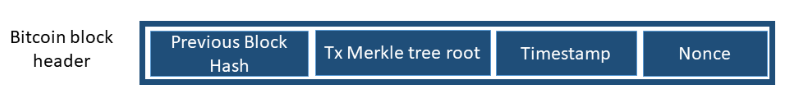
\includegraphics[width=1.0\linewidth]{bitcoincabecera.png}
    % \label{fig:enter-label}
\end{figure}
}

\frame{
\frametitle{Merge-Mining}
\begin{block}{Definición}
    Técnica que permite minar dos o más criptomonedas al mismo tiempo sin gastar poder de cómputo extra.
\end{block}
\pause
\begin{itemize}
    \item Misma tasa de emisión de bloques.
    \item Mismo algoritmo de prueba de trabajo(\textit{PoW}).
    \item Un bloque de la primaria y uno o ninguno de la secundaria.
    \item Distintas dificultades de minado (\textit{target})
\end{itemize}
}

\frame{
\frametitle{Árboles de Merkle}
\begin{figure}
    \centering
    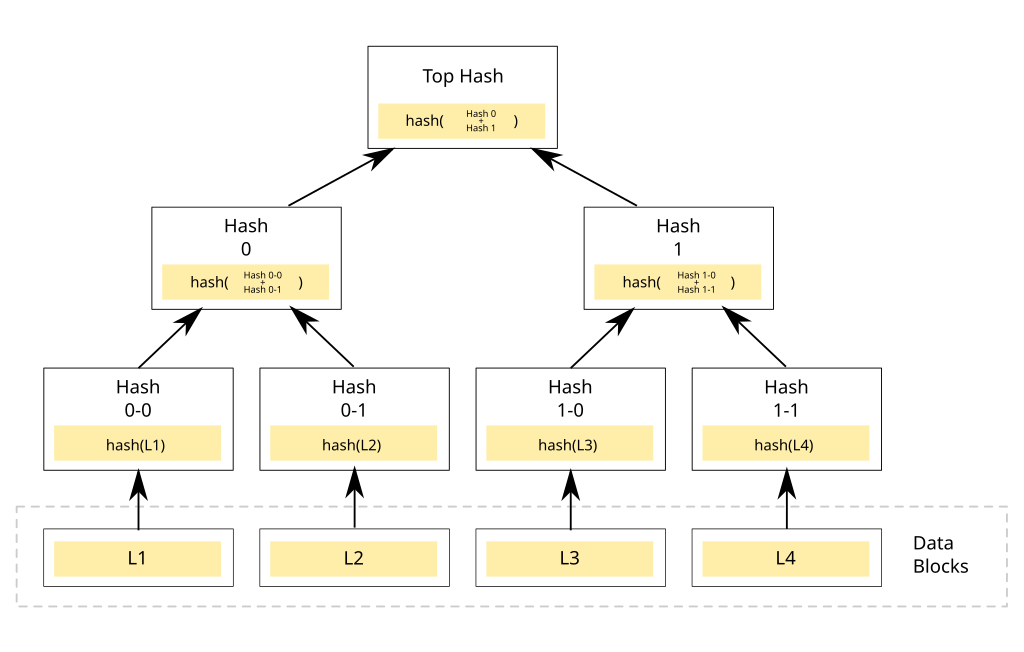
\includegraphics[width=1.0\linewidth]{merkleTree.png}
    % \label{fig:enter-label}
\end{figure}
}

\frame{
\frametitle{Las pruebas SPV}
Verificar que una transacción está incluida en la blockchain.\newline

Para verificar que una transacción pertenece a un bloque, el nodo SPV solo necesita la ruta Merkle (\textit{Merkle Path}) para reconstruir la \textit{Merkle Root}.\newline
\begin{block}{RSK}
    Puede verificar que la relación está hecha sin necesidad de leer el bloque de Bitcoin.
\end{block}
}

\frame{
\frametitle{Las pruebas SPV}
\begin{figure}
    \centering
    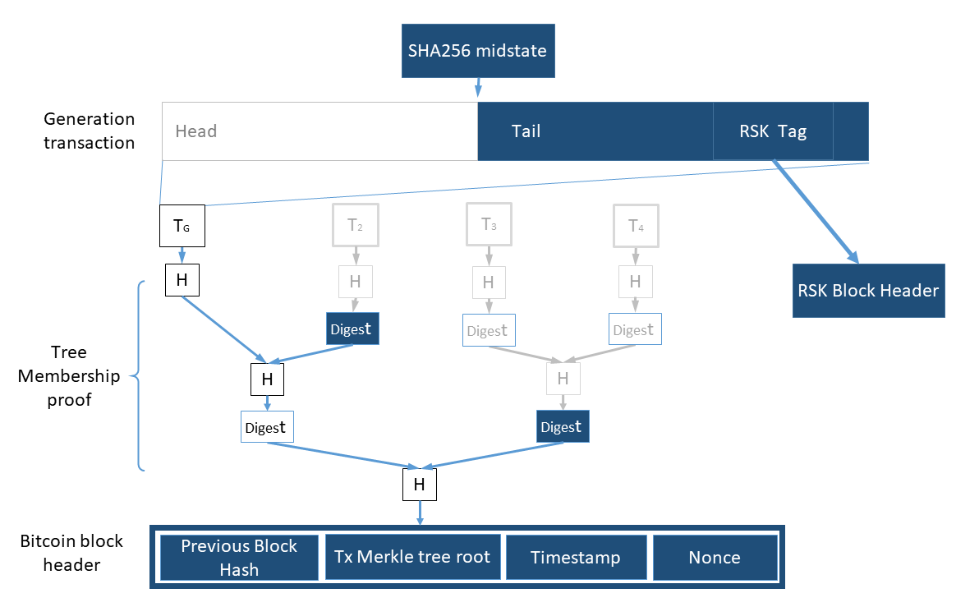
\includegraphics[width=1.0\linewidth]{spvproof.png}
    % \label{fig:enter-label}
\end{figure}
}

\frame{
\frametitle{Como se relacionan las cadenas}
Lograr una relación bidireccional entre cadenas
\begin{block}{RSK}
    \begin{columns}
        \column{0.4\textwidth}
        \begin{figure}
            \centering
            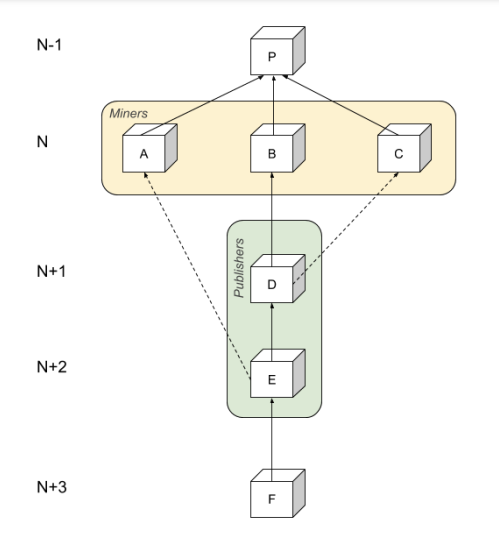
\includegraphics[width=0.9\linewidth]{minadoRSK.png}
            % \label{fig:enter-label}
        \end{figure}
        \column{0.6\textwidth}
        \begin{itemize}
            \item A, B y C comparten el mismo padre P.
            \item B es el \textit{best block}, A y C son \textit{siblings}.
            \item D incluye a C como \textit{uncle}. E incluye a C como \textit{uncle}.
            \item F es un nuevo bloque agregado a la mainchain
        \end{itemize}
    \end{columns}
\end{block}
\footnotetext{Medina, M. G. (2021) Un estudio del rendimiento del minado Bitcoin en escenarios de Merged Mining}
}

\frame{
\frametitle{Jerarquia de targets}
\begin{block}{Definición}
    Es la dificultad definida para una PoW. Más alta implica menos dificultad.
\end{block}\pause

Resolver el problema de la cadena principal (mayor costo) y paralelamente la solución para la secundaria (menor costo).\newline

Las soluciones para la red secundaria son 20 veces más comunes, son validos para ella pero no para la principal


}

\frame{
\frametitle{Etiquetas RSK}
\begin{center}
    \texttt{RSKBLOCK:<blockHash>}
\end{center}
Puede estar: \it{codebase} ó \it{Output of the generation transaction}\newline\pause

\textbf{Consideraciones:}
\begin{itemize}
    \item Luego de la etiqueta debe haber menos de 128bits.
    \item No debería haber etiqueta en los bits libres.
    \item Pueden aparecer por casualidad, ponerlas al final.
    \begin{itemize}
        \item codebase: No es un problema si está la etiqueta \texttt{ExtraNonce2}
    \end{itemize}
\end{itemize}
Por cuestiones de tamaño suelen estar en la codebase o entre los últimos 4 de la transacción. La segunda permite generar prueba SPV.
}

\frame{
\frametitle{Seguridad de la Merge-Mining(RSK)}

En general los sistemas de consenso brindan seguridad sobre teoría de juegos y caos.\newline

\textbf{Ataques:}
\begin{itemize}
    \item Ataque irracionales de $2^{80}$ operaciones en 30 segundos
    \item Ataque racional de $2^{69}$ operaciones. 
\end{itemize}
}

\frame{
\frametitle{Posibles lugares de ataque}
Usa un truco criptográfico no estándar para comprimir la transacción.
\begin{itemize}
    \item Solo trasmite su final
\end{itemize}
Requiere asumir una propiedad fuerte de SHA-256, \textit{freestar collision}. Poder comenzar desde estados intermedios sin tener coliciones en estos.
\noindent\rule{\textwidth}{1pt}\pause

No hay beneficios por encontrar colisiones a bloques. Tampoco por minar bloques antiguos. Existe la capa de seguridad dada por la PoW. 

}

\frame{
\frametitle{Cierre:}
\begin{itemize}
    \item Aprovechar la seguridad de Bitcoin.
    \item Extender los comportamientos de una red (sin modificar su protocolo)
    \item No necesitar una red de mineros dedicada.
    \item El minado resulte más atractivo.
\end{itemize}
}
\end{document}